\documentclass{final_report}
\usepackage[backend=biber,
            sorting=none,
            language=british]{biblatex} %create bibliography
\usepackage{graphicx}
\usepackage{lastpage}
\usepackage{verbatim}
\usepackage{fancyvrb}
\usepackage[shortlabels]{enumitem} %change list formatting
\usepackage[pdftex,
            colorlinks,
            breaklinks=true,
            linkcolor={black},
            citecolor={black},
            urlcolor={blue!60!black},
            pdfauthor={George Honeywood},
            pdftitle={Final Year Project --- Interim Report}]{hyperref} 

% prevent long urls in the in the bibliography from overfilling (weird breaks are preferred)
\setcounter{biburlnumpenalty}{9000}
\setcounter{biburllcpenalty}{9000}
\setcounter{biburlucpenalty}{9000}

\setlist[itemize]{noitemsep, nolistsep} %make lists take up less room
\setlist[enumerate]{noitemsep}

\addbibresource{../sources.bib}

%%%%%%%%%%%%%%%%%%%%%%
%%% Input project details
\def\studentname{George Honeywood}
\def\reportyear{2022}
\def\projecttitle{Offline HTML5 Maps Application}
\def\supervisorname{Reuben Rowe}
\def\degree{BSc (Hons) in Computer Science}
\def\fullOrHalfUnit{Full Unit} % indicate if you are doing the project as a Full Unit or Half Unit
\def\finalOrInterim{Interim Report} % indicate if this document is your Final Report or Interim Report

\begin{document}

\maketitle

%%%%%%%%%%%%%%%%%%%%%%
%%% Declaration

% \chapter*{Declaration}

% This report has been prepared on the basis of my own work. Where other published and unpublished source materials have been used, these have been acknowledged.

% \vskip3em

% Word Count: 

% \vskip3em

% Student Name: \studentname

% \vskip3em

% Date of Submission: 

% \vskip3em

% Signature: GH

% \newpage

%%%%%%%%%%%%%%%%%%%%%%
%%% Table of Contents
\tableofcontents\pdfbookmark[0]{Table of Contents}{toc}

%%%%%%%%%%%%%%%%%%%%%%
%%% Your Abstract here

\begin{abstract}
    Although online web maps are commonplace, offline maps are a valuable niche that are useful in certain situations, such as on mobile devices with limited data, or when roaming abroad. There are limited options in this space that are cross-platform, which I hope my project can resolve through the nature of it being provided as a progressive web app (PWA).

    In this project I aim to build an offline maps application based on OpenStreetMap data. The user should be able to download map data for their area of interest, then view it by panning and zooming, like a traditional online slippy map. Time permitting, I may also add additional features that require an internet connection, like routing and Wikipedia integration. Through this project I hope to learn about how you project map data into a rendered map. It will also teach me how to successfully develop a medium-sized application.
\end{abstract}
\newpage

% for final report:
%%%%%%%%%%%%%%%%%%%%%%
%%% Project Spec

% \chapter*{Project specification}
% \addcontentsline{toc}{chapter}{Project specification}
% Your project specification goes here.

%%%%%%%%%%%%%%%%%%%%%%
%%% Introduction
\chapter{Introduction}

The OpenStreetMap project began in 2004, with the aim of creating a free world map~\cite{RAMM:2011}. Since then, it has met and surpassed its goals, becoming a mature, global dataset, edited by both volunteers, and corporations alike. As of late 2022, an average of 6,000 contributors edit the map daily, with more than 9 million registered in total~\cite{OSMStats}. In contrast to how cartography is traditionally carried out, OSM contributors tend to not use any specialized equipment, instead using tools like GPS and aerial imagery to create the map. The barrier of entry is low by design, making it easy for new mappers to get started. This sometimes results in inaccurate, or even vandalistic edits being made, but the community usually spots and reverts bad edits quickly.

I have personally been involved in the OpenStreetMap project since creating an account on the 25th of May 2019. This was initially as I was using an OSM based map, and noticed that a new-build estate near my house was missing. Hence, \href{https://www.openstreetmap.org/changeset/70609319}{I added it}, and this led me down the rabbit hole of wanting to add all the missing features around me. Since then, I have been a regular contributor, with currently almost \href{https://www.openstreetmap.org/user/GeorgeHoneywood}{2,000 changesets} made over 341 separate days. I have also made some code contributions to the Every Door mobile editor, specifically adding support for viewing an element's history~\cite{every-door}. 

Although online OpenStreetMap-based web maps are very popular, offline maps are much less of an explored field. On the Android platform, you have a few options for offline maps, such as the venerable OsmAnd~\cite{osmand}, Organic Maps (FOSS fork of Maps.me~\cite{maps.me}), and the proprietary Magic Earth~\cite{magic-earth}. On desktop, the available options are more sparse. KDE Marble is one option~\cite{kde-marble}, but it seems like the offline experience is an afterthought. It allows you to download pre-rendered Mapnik Carto style tiles, and this is limited to above zoom level 16, so fine details are not visible (\href{https://openstreetmap.org}{openstreetmap.org} renders tiles down to zoom level 19). This approach of downloading rendered raster tiles is also not very scalable, as there quickly becomes a huge number of images that need to be downloaded, and these images take up significant storage space. For example, I attempted to download the tiles for Cornwall, UK, in KDE Marble, and it would have had to fetch 58,928 tiles just for between zoom levels 11 and 16, equating to an estimated download size of 749 MB\@. This method is also explicitly prohibited by the OpenStreetMap Foundation's Tile Usage Policy, which states that ``In particular, downloading an area of over 250 tiles at zoom level 13 or higher for offline or later usage is forbidden.''~\cite{OSMF-tile-usage-policy}. This is because rendering map tiles is computationally expensive, and the OSMF is run with a limited budget.

Another option is the OpenStreetMap API itself~\cite{osm-api-wiki}. This is more promising for offline usage, as it allows you to download vector data that can be stored more efficiently than raster images. However, the API is not designed for this use case --- it is an interface specifically for map editor programs to use. As such, you can only download small geographical areas at a time, and the data is not stored in an optimal format for rendering. For example, complex structures, such as buildings with internal courtyards, are represented in OSM with multipolygon relations, which are difficult to parse and render correctly when using raw OSM data. An additional barrier to using the editing API is that its Terms of Use explicitly prohibit read only applications~\cite{OSM-editing-API-usage-policy}.

Cruiser follows a more promising approach~\cite{cruiser}. Instead of downloading rendered image tiles, it uses prebuilt vector map files, in the Mapsforge binary format~\cite{mapsforge-format}. This is much more space efficient --- the whole of England is an 805 MB download. It is also much less difficult to host, as you don't need a powerful server to render the raster map tiles on the fly. One possible issue with this approach is that this may be too much data to store in a HTML5 web application, and this is something I will have to explore further.

Offline maps are a niche market, as desktop computers tend to always have an internet connection, and on mobile devices data is cheap enough to allow downloading some small vector or raster map tiles. Hence, the main use-case for an offline HTML5 map would be for when an internet connection is either prohibitively expensive or not available at all. This could be when roaming abroad, or when in an area without LTE coverage. As such, it makes sense to make support for mobile devices a priority, as they are the most likely to be in these situations.

From this project I hope to learn how map data actually becomes a rendered map, as currently my understanding of this process is limited. I also hope to learn more about offline HTML applications, as I think that this type of web app has lots of room to become popular in the coming years. There are lots of apps on my phone that I think could be replaced by a PWA (progressive web app).


%% these sections have basically been covered in the introduction.
%% maybe it would be good to split the introduction out.
% \section{Issues}
% \section{Motivation}

\section{Literature review}

Whilst researching my primary source for information about the OpenStreetMap project was \emph{OpenStreetMap — Using and Enhancing the Free Map of the World}, by \textcite{RAMM:2011}. This provided a good foundation of knowledge  that supplemented information that I have picked up over the years due to being involved with the project. Some sections were a little out of date, especially the sections on editors and tools for mappers. Notably the online editor referred to here, Potlatch, is no longer available, being superseded by iD in 2013.

For more up to date or specific information I often relied on the OpenStreetMap Wiki~\cite{osm-wiki}, which provides a helpful reference for both OSM specific information and other GIS adjacent topics. These include general information about map projections~\cite{osm-wiki-mercator}, and details about the Z/X/Y tiling scheme that is common for web maps~\cite{osm-wiki-tile-names}.

When it came to implementing the project, MDN Web Developer documentation proved invaluable~\cite{mdn}. They provide an excellent reference on how to use many web APIs, with detailed usage guides included. In particular, the information about the Canvas API~\cite{mdn-canvas-api}, and Service Workers~\cite{mdn-service-workers} was very useful, as these were technologies that I was not familiar with.

\section{Aims and objectives}

Here I will list some specific features that I would like to implement in the project. These are not fixed, and some may not be implemented, or others added in their place.

\begin{itemize}
    \item Download vector map data for a user-provided region (preferably at least as large as a UK county), allowing the user to browse the map offline
    \item Allow the user to pan and zoom the map. They should be able to zoom out to the view the full extent of the downloaded data.
    \item Provide a search functionality, using the Nominatim API
    \item Allow the user to route between two points, which could be implemented using OSRM, GraphHopper or Valhalla
    \item When an OSM element has been tagged with a reference to a Wikipedia article, it should show a description from Wikipedia
    \item Allow the user to save and name markers for later use
    \item When online, the application should allow the user to browse a map without having to first download any data. This could be done using raster tiles.
\end{itemize}

\section{Milestones}

% FIXME: presumably this should be in past tense

Following a timeline will help my project proceed without any major unexpected delays, and will give me targets to aim for. At the beginning of term 1 I focussed on exploring any risky areas or technologies that I was unsure about. This helped answer any large questions early on in the process.

\begin{enumerate}
    \item Report on offline HTML5 technologies. Used this to discover whether it is possible to download \& store a large amount of vector map data (>100 MB) for later rendering.\label{item:deliverable:offline-html}
    \item Proof of concept basic offline HTML5 app. Used this to discover any limit of how files can be stored for offline use.\label{item:deliverable:basic-offline-app}
    \item Report on the different ways  that the program could get OpenStreetMap data. One possibility is the Mapsforge format, or it could use the OSM editing API\@. This helped mitigate risk of using a technology that is not suitable for the project.\label{item:deliverable:osm-data}
    \item Report about how map projection works. Specifically the mathematics behind projecting the data that is produced by OpenStreetMap. This ensured that I understood this key concept.\label{item:deliverable:map-projection}
    \item Proof of concept that took some way made up of latitude longitude pairs and draws a line onto a canvas.\label{item:deliverable:draw-line}
    \item Make proof of concept~\ref{item:deliverable:draw-line} interactive; allow the user to pan and zoom the map. This should be done with the scroll wheel on desktop and pinch zooming on mobile.\label{item:deliverable:pan-zoom}
    \item Proof of concept that loads some actual OSM data using the technology that I decided upon in deliverable~\ref{item:deliverable:osm-data}.\label{item:deliverable:load-osm-data}
    \item Thoroughly test the application on mobile, as this will likely be the main use case for an offline map.\label{item:deliverable:mobile-testing}
    \item Add online search functionality, using the Nominatim API.\label{item:deliverable:search}
    \item Add online routing functionality, using OSRM, GraphHopper or Valhalla.\label{item:deliverable:routing}
    \item Show point of interest information from Wikipedia, when an OSM element has been tagged to allow this.\label{item:deliverable:wikipedia}
    \item Add the ability to save and name markers for later use.\label{item:deliverable:markers}
    \item Allow the user to browse the map without first downloading data when online. This could be done using raster tiles.\label{item:deliverable:online}
\end{enumerate}

\subsection{Term 1}

\begin{itemize}
    \item \textbf{Week 3 (2022/10/03)}: Report~\ref{item:deliverable:offline-html}.
    \item \textbf{Week 4 (2022/10/10)}: Proof of concept~\ref{item:deliverable:basic-offline-app} \& report~\ref{item:deliverable:osm-data}.
    \item \textbf{Week 5 (2022/10/17)}: Report~\ref{item:deliverable:map-projection} \& proof of concept~\ref{item:deliverable:draw-line}.
    \item \textbf{Week 6--7 (2022/10/24)}: Proof of concept~\ref{item:deliverable:pan-zoom}.
    \item \textbf{Week 8--9 (2022/11/07)}: Proof of concept~\ref{item:deliverable:load-osm-data}.
    \item \textbf{Week 10--11 (2022/11/21)}: Prepare for the interim report, and presentation.
\end{itemize}

\subsection{Term 2}

\begin{itemize}
    \item \textbf{Week 1--2 (2023/01/10)}: Integration of the above proof of concepts into the final program.
    \item \textbf{Week 3--4 (2023/01/24)}: Deliverable~\ref{item:deliverable:mobile-testing}.
    \item \textbf{Week 5 (2023/02/07)}: Prepare an initial draft for the final report.
    \item \textbf{Week 6--7 (2023/02/14)}: Add support for further features, such as deliverables \ref{item:deliverable:search}, \ref{item:deliverable:routing}, \ref{item:deliverable:wikipedia}, \ref{item:deliverable:markers} and \ref{item:deliverable:online}.
    \item \textbf{Week 8 (2023/02/28)}: Evaluate the solution so far, and decide whether to extend the project further, if time permits.
    \item \textbf{Week 9--11 (2023/03/27)}: Prepare for the final report.
\end{itemize}

\chapter{Research}

\section{Basic HTML5 technologies}

% write another report here, only on basic stuff.

\section{Offline HTML5 applications}\label{sec:offline-html-applications}

In order to create an offline HTML5 map application, I will first have to research how offline HTML5 applications work, and what technologies I'll need to become familiar with.

There are various different APIs that one can use to store data in an offline HTML5 application, such as IndexedDB, the File and Directory Entries API~\cite{w3c-file-directories-api}~\cite{mdn-file-directories-api} and localStorage. localStorage will likely not be appropriate for my use case, as it is designed for only small amounts of data. There is also the Application Cache, but this has been deprecated, and support has been removed from all major browsers~\cite{whatwg-application-cache}~\cite{mdn-application-cache}. Therefore, the Application Cache will not be suitable for a new application.

If I am to process and use a large precompiled map data format, like mbtiles~\cite{mbtiles-spec} or Mapsforge~\cite{mapsforge-format}, using the File and Directory Entries API will likely be more appropriate. For optimal performance, it may be necessary to have a loading step, I transform from one of these formats into the IndexedDB, for usage by the app. Hopefully this step can be avoided, as it would not be ideal to have multiple copies of the data, particularly on space constrained devices.

\begin{quote}
    ``The File and Directory Entries API simulates a local file system that web apps can navigate around. You can develop apps that can read, write, and create files and directories in a sandboxed, virtual file system.''
    
    \footnotesize{--- \fullcite{mdn-file-directories-api}}
\end{quote}

Another benefit of the File and Directory Entries API~\cite{w3c-file-directories-api}, is that it has the ability to act like a local file system. This would allow my app to have a flow like:

\begin{itemize}
    \item User opens the webapp
    \item Selects map to download from list (or as an enhancement by zooming in on desired region on a low detail world map)
    \item App downloads the map file to sandboxed filesystem
    \item User goes offline
    \item Map rendered from this internally stored file
\end{itemize}

A flow like this makes sense from a user's perspective, as it follows a similar paradigm to other offline map viewers, like Organic Maps or OsmAnd (as discussed in the initial plan).

If there are issues with using the File and Directory Entries API, for example file size limits in certain browsers, it should be possible to use the plain File API instead~\cite{w3c-file-api}. The File API allows access to read single files from a user's local filesystem. Importantly for my use case of loading a large map file from a user's disk, we cannot store the entire file in RAM at once. Usefully the File API provides a \texttt{.slice()} method, which allows you to work with a smaller subsection of the file. This will likely be important to avoid out-of-memory (OOM) errors.

Using the plain file API will however come at a detriment to the user flow. Instead of being able to select and download a map within the app, the user will have to download the map file themselves, then point the app to the map file they have downloaded. This is not a major issue, but it would be preferable to have this process handled without user interaction.

Unfortunately the Files and Directory Entries API has limited support in Firefox~\cite{mdn-file-directories-api-limitations}. Critically \texttt{window.requestFileSystem()} is not supported, and this is the function that you call to gain access to a virtual filesystem. In Firefox this API can only be used through an \texttt{<input>} element, or drag and drop. This is an issue as for my application, the app would need to be able to create the virtual filesystem programmatically.

\begin{quote}
    ``Content scripts can't create file systems or initiate access to a file system.''

    \footnotesize{--- \fullcite{mdn-file-directories-api-limitations}}
\end{quote}

Hence, if I wish to use the File and Directory Entries API, which would provide a smoother user journey, I would not be able to support Firefox. For my application I think it is more important to support Firefox than have perfect UX --- so I will settle on the compromise of the user having to select the desired map file on each start, via the file picker. This will be an irritation, but unfortunately there is no widely compatible way to use a sandboxed/virtual filesystem in the browser.

One benefit of storing the map file outside the browser is that my application will not have to deal with the browser not allocating it enough storage quota for the file. For example in Chrome, you must use the Quota Management API to request persistent storage space to use~\cite{gd-offline-html5-storage}, which will prompt the user to accept the request.

Another option is to use the Cache API, which is part of Service Worker specification~\cite{w3c-service-workers-caches}, and has good cross-browser support. It has a simpler interface that should work for the application --- a pair of a request and a response object are stored, and you get a cached version of the response by providing a similar request. 

To determine which will be the best choice for the application, I will produce proof of concepts that employ the File API and the Cache API\@.


\section{Using the HTML5 canvas}

The HTML5 Canvas provides another dimension to web applications, where bitmap animations or other data can be displayed interactively.

\begin{quote}
    ``HTML5 Canvas is an immediate mode bitmapped area of the screen that can be manipulated with JavaScript. Immediate mode refers to the way the canvas renders pixels on the screen. HTML5 Canvas completely redraws the bitmapped screen on every frame by using Canvas API calls from JavaScript.''

    \footnotesize{--- \fullcite{fulton2013html5}}
\end{quote}

So, in my application, the canvas is what the map will be ``drawn'' to. The canvas API provides different interfaces that you can use, known as rendering contexts~\cite{mdn-canvas-api}. For simple 2D drawing, there is the \texttt{CanvasRenderingContext2D} interface. For more intensive 2D and 3D workloads, there is the GPU accelerated \texttt{WebGLRenderingContext}, which uses an OpenGL-like system of vertex and fragment shaders~\cite{mdn-web-gl}. This is what some existing vector web map libraries use, like Mapbox's GL JS~\cite{mapbox-gl-js}.

In the long run, the \texttt{WebGLRenderingContext} would be the best choice in terms of efficiency and performance, as it is hardware accelerated. However, the \texttt{Canvas\-Rendering\-Context2D} has a far simpler API, so it makes sense to use it here.

The simplest operation I will need to use the canvas for is drawing the outlines of polygonal shapes. Note that on the canvas, \texttt{(0, 0)} is at the top left. To begin drawing, you first need to get an instance of \texttt{Canvas\-Rendering\-Context2D}, which is done by calling \texttt{const ctx = canvas.getContext(``2d'')} on some canvas element in the DOM\@. To start on the polygon, call \texttt{ctx.beginPath()} to create a new path, that you then add data to using the \texttt{ctx.lineTo(x, y)} method. If required, you can also call \texttt{ctx.moveTo(x, y)} to have the line jump from one spot to the next. Once you have made your \texttt{.moveTo()} and \texttt{.lineTo()} calls, you then execute \texttt{ctx.stroke()} to render the line out.

Another operation I will need to perform to create a styled map is creating ``filled'' polygons. For example, \href{https://openstreetmap.org}{openstreetmap.org} renders buildings with a brown infill and a darker outline. This is achieved on the canvas in a very similar way to the polygon outline, but instead of calling \texttt{ctx.stroke()} to render the path, you call \texttt{ctx.fill()}. To control the colour, you set \texttt{ctx.fillStyle} to some desired value.

To render names of points of interest and ways to the map, I will need a method to write text to the canvas. This can be done using \texttt{ctx.fillText(`string', x, y)}~\cite{mdn-canvas-draw-text}. Unfortunately this does not make provisions for drawing text at an angle, which would be useful for drawing names of roads or boundaries, where the name follows the curve of the geometry. However, you can use the \texttt{ctx.rotate(angle)} to achieve a similar result, albeit with some more complexity~\cite{mdn-canvas-rotating}.

Another useful method for drawing a map will be the \texttt{ctx.measureText(`string')} method, which returns the pixel size that the text will be drawn at. This information can be used to prevent labels on the map overlapping, by storing each of the previously drawn labels' boundary boxes, and preventing new labels from being drawn if they are colliding.

Finally, the \texttt{Path2D} interface may be useful for my application~\cite{mdn-canvas-path-2d}. It allows you to save a path, meaning you can stroke and fill some geometry, without having to draw the path twice. Hence, it should give an efficiency boost. You use it like so:

\begin{lstlisting}
const ctx = canvas.getContext('2d');

let path = new Path2D();
path.rect(5, 5, 20, 20);

ctx.stroke(path);
ctx.fill(path);
\end{lstlisting}


\section{OpenStreetMap data sources}\label{sec:osm-data-sources}

In order to produce a map using OpenStreetMap data, you first need to decide which source/format of data to use. Traditionally, for this project, students use the OpenStreetMap editing API\@. This however, has a number of limitations, some of which I have already discussed in the project plan.

\begin{itemize}
    \item It is designed for map editing applications, and the terms of service explicitly prohibit read-only uses~\cite{OSMF-tile-usage-policy}.
    \item You can only download a relatively limited geographical area, usually only around 2 km\textsuperscript{2}. This has the effect that you will not be able to zoom out to see a large area, such an entire country~\cite{osm-wiki-limited-area}.
    \item Complex structures (like buildings with internal courtyards) represented in OpenStreetMap as multipolyons require extensive parsing and validation to correctly display.
\end{itemize}

For online maps, it is common to use either raster or vector ``map tiles''. Raster map tiles are usually 256\(\times{}\)256 \texttt{.png} files, rendered by a Mapnik server. These tiles are named according to their zoom level, and an \(x\) and \(y\) value, where \(x\) and \(y\) are offsets from the top left most tile~\cite{osm-wiki-tile-names}. Raster tiles, however, are not particularly appropriate for offline usage, as you have to request an extremely large amount of tiles, especially when you approach high zoom levels. For example if you downloaded 4 tiles at zoom 10, you would need to download 16 at zoom 11, 64 at zoom 12, and 262144 at zoom 18. This behaviour is unacceptable as rendering tiles is computationally expensive for the OpenStreetMap Foundation, and the size of these tiles adds up.

Vector tiles use a similar scheme, with tiles also being served at Z/X/Y addresses. The key differentiator is that instead of rendered images, vector data is served to clients, and it is up to the clients to render this data into a map. This gives the clients flexibility in how they can choose to display the data, such as the colours, labels, and line thicknesses. This is usually done through stylesheets. As vector data does not pixelate like raster images, you can ``overzoom'' on vector tiles, meaning you do not have to serve tiles to such high zoom levels. One of the most popular formats for vector map tiles are Mapbox Vector tiles. These use the Google Protobuf format to store the vector data.

Vector tiles make a more appropriate offline format than raster tiles, due to their ability to ``overzoom'', and that vector data can be stored more efficiently. Unfortunately it is still not particularly suited to offline usage, as with raster tiles, you need to download many tiles to cover a large region.

Therefore, it makes sense to use a dedicated storage format, that is designed to provide map data for offline applications. The OpenStreetMap Wiki provides a number of possible options for this purpose~\cite{osm-wiki-offline}. The most popular choices are mapsforge~\cite{mapsforge}, which is used by many applications~\cite{apps-using-mapsforge}, and MBTiles (by Mapbox)~\cite{mapbox-mbtiles}. Unfortunately, as the MBTiles format is based on an SQLite database, it can't easily be used in a HTML5 app.

Mapsforge, on the other hand, uses a custom binary data format~\cite{mapsforge-format}. Mapsforge only provide libraries for the Java language and the Android platform. There is a partial implementation available of a parser written in JavaScript, which only supports decoding the headers and other metadata. Hence, to use this format for my project, I would need to implement my own parser, which would add substantial complexity. I may also need to tackle issues with memory usage, as parsing and rendering the file will require random access within it --- meaning loading the whole file into an \texttt{ArrayBuffer} or some similar structure. Using the \texttt{Blob.slice()} method in JavaScript may allow me to work around this issue to some degree.

If parsing the Mapsforge binary files is too complex, I can scale back the project to using the OSM Editing API\@. This will require less parsing work, but will still have plenty of issues to overcome in terms of rendering.


\section{Projecting map data}\label{sec:projecting-map-data}

The core of this project is being able to render a map. This in its most basic form means being able to take coordinates, which represent a position on the sphere-like body that is the earth, and placing these on a two-dimensional plane. This process is known as map projection~\cite[5]{canters2002small}.

OpenStreetMap uses the WGS84 coordinate reference system (EPSG:4326) to represent the positions of the nodes that make up its data~\cite{osm-wiki-wgs84}. GPS uses this CRS, and it is a popular standard~\cite{epsg.io-epsg:4326}.

If you were to naively place coordinates from the WGS84 system on to a graph, you would get a ``plate carrée'' projected map. This projection is a form of the equirectangular projection, where the standard parallel \(\phi_1 = 0\). In plate carrée, lines of longitude are straight, vertical and equidistant, and lines of latitude are similar, albeit horizontal. Although all map projections are compromises between conformality (preservation of angle) and preservation of area, plate carré does not preserve either, meaning it is not particularly well-used.

Hence, OpenSteetMap uses the ``Web Mercator'' projection (also known as Spherical Mercator, WGS 84/Pseudo-Mercator, Google Web Mercator, EPSG:3857). This projection is almost conformal, meaning that (local) angles on the map are the same as angles on the ground, even if lengths are not preserved~\cite{carto-implications-of-webmercator,}. It deviates from normal Mercator in that its calculations are based on the earth being a true sphere, rather than ellipsoidal. The benefit of this is that the calculations for converting between WGS84 latitude/longitude coordinates, and Web Mercator are simpler than normal Mercator~\cite{ugrc-earth-not-round}.

So, to convert from latitude/longitude coordinates to Web Mercator, we can use equations 7--1a \& 7--2a from \textcite[41]{snyder1987map}, where \(\lambda{}\) is longitude and \(\phi{}\) is latitude, both in degrees:

\[x = \frac{\pi R(\lambda^\circ - \lambda^\circ_0)}{180^\circ} \]

\[y = R \ln \tan \left( 45^\circ + \frac{\phi^\circ}{2} \right) \]


\chapter{Proof-of-concept development process}

% talk about proof of concepts here!
% little write up of how each works, and what it achieves

As part of the development process, I have created a number of proof-of-concepts, that each build on each other. These have helped me to understand, test and evaluate various technologies that I could use to build the final application.

\section{Simple offline HTML5 app}

{ \hfill \footnotesize Source in \texttt{proof-of-concepts/1-offline-html5}}

My first proof of concept was a basic offline HTML5 application, employing the techniques that I researched in Section~\ref{sec:offline-html-applications}. Since the \texttt{Application Cache} has been deprecated, the accepted way to create an offline HTML5 app is to use Service Workers~\cite{w3c-service-workers-caches}. The concept behind this is that the Service Worker intercepts all HTTP requests that are made on the website, and can then respond to this request with a result from a prepopulated cache.

In addition to creating an offline HTML5 app, I also learned how to store a large binary blob. This will be necessary for my project, as this is how the map data will be stored. To this end I looked at using both the Service Worker cache, and the File API\@.

The File API works like a traditional file picker --- allowing the user to choose some file from their local filesystem~\cite{w3c-file-api}. This is useful, but does not provide an excellent user experience. For example the user would have to download a map file to some location on their computer, then select it in the file picker every time they want to view a map. This violates Nielsen's ``Recognition, not recall'' heuristic~\cite{nielsen-heuristics}, as the application should work without the user having to remember where they saved the map file.

Therefore, it is preferred to use the Service Worker cache method, where you store the file inside the web browser's cache. Storing binary blobs works like using the Service Worker cache for normal website resources:

\begin{lstlisting}[caption=Using the Service Worker cache]
self.addEventListener('install', (event) =>  event.waitUntil(
        addResourcesToCache(['/index.html', '/blob.map']) // prepopulate cache
));

const cacheFirst = async ({ request }) => {
    const responseFromCache = await caches.match(request);
    if (responseFromCache) { // try to get the resource from the cache
        return responseFromCache;
    }

    return new Response('could not retrieve from cache', {
            status: 408,
            headers: { 'Content-Type': 'text/plain' },
        });
};

self.addEventListener('fetch', (event) => event.respondWith(
        cacheFirst({request: event.request})
));
\end{lstlisting}

\section{Rendering geometry to a canvas}

{ \footnotesize Source in \texttt{proof-of-concepts/2-rendering-a-way}, or online demo at \href{https://files.george.honeywood.org.uk/2-rendering-a-way/}{\nolinkurl{files.george.honeywood.org.uk/2-rendering-a-way/}}.}

My second proof of concept was to draw some geographical data on to the canvas. As a first step, I had to acquire some data to project. As this was a simple proof of concept I decided to use the GeoJSON format, which a popular standard for representing geodata, in a fairly human-readable format. The main reason I chose it was that it is easier to parse in JavaScript than the XML data that the OpenStreetMap API provides~\cite{osm-api-wiki}. For my first test, I attempted to render the boundary of Egham, which is currently \href{https://www.openstreetmap.org/way/666914693}{way 666914693}. To convert XML data from OpenStreetMap I used the online \texttt{geojson.io} tool, which allows you to import OSM XML and export GeoJSON~\cite{geojson.io}.

The main challenge I wanted to solve in this proof of concept was projecting the data. This stage is necessary, as OpenStreetMap data comes in the WGS84 CRS, and while this can be naively plotted on a graph as (x,y) coordinates, this would result in the ``plate carrée'' projection, as detailed in Section~\ref{sec:projecting-map-data}. The ``plate carrée'' projection is not particularly desirable, as it does not have any useful properties like conformality (preservation of angle) or preservation of area. Hence, for my application I chose to use Web Mercator, which preserves conformality, and is the de facto standard for web maps.

Initially, I attempted to use the algorithm from \textcite[41]{snyder1987map}, as shown in Section~\ref{sec:projecting-map-data}. Unfortunately I had some issues with getting these equations to produce reasonable results. Therefore, I turned to the OpenStreetMap Wiki, which helpfully provides a reference for transforming WGS84 data into the Web Mercator projection~\cite{osm-wiki-mercator}. I translated the C example into TypeScript, and it correctly projected the data.

\begin{lstlisting}[caption=Projecting to Web Mercator]
const RADIANS_TO_DEGREES = 180 / Math.PI;

// calculate x/long
const x = long;
// calculate y/lat
const y = Math.log(Math.tan(
    (lat / RADIANS_TO_DEGREES) / 2 + Math.PI / 4
)) * RADIANS_TO_DEGREES;
\end{lstlisting}

\begin{figure}[ht]
    \centering
    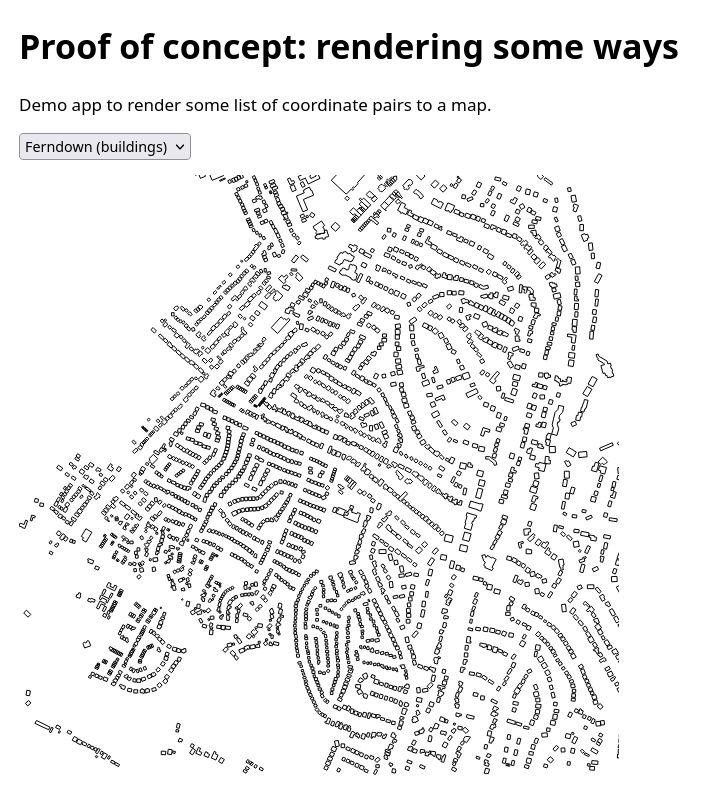
\includegraphics[width=0.7\textwidth]{../proof-of-concepts/2-rendering-a-way/screenshots/ferndown-buildings.png}
    \caption{Rendering some GeoJSON data to the canvas}
\end{figure}\label{fig:rendering-geometry}

This proof of concept was entirely static, with the viewport and zoom level hardcoded into the program. To make the implementation simpler I wrote a function that scaled all the coordinates to be around (0,0), so that I didn't have to handle offsetting the viewport.

\section{Adding interactivity --- panning and zooming}

{ \footnotesize Source in \texttt{proof-of-concepts/3-panning-and-zooming}, or online demo at \href{https://files.george.honeywood.org.uk/3-panning-and-zooming/}{\nolinkurl{files.george.honeywood.org.uk/3-panning-and-zooming/}}.}

The third proof of concept heavily built upon this second --- with the goal of adding interactivity in the form of panning and zooming. As being mobile friendly is a priority for my project, I made sure to add touch controls once I had it working with mouse events.

The first part I tackled was the zooming. This turned out to be as simple as multiplying each projected coordinate by some scale factor, which I was already doing in the previous proof of concept. To modify this scale factor, the user can use the +/- buttons, the mouse scroll wheel, or a pinch gesture on a touch device. Pinch gestures were the most challenging to implement, as you have to handle and interpret \texttt{Touch} events for each separate finger on the screen.

Panning also turned out to be relatively easy --- my implementation involved adding some offsets to the projected and scaled coordinates in the latitude and longitude axis. What was more complicated was having the map zoom about some arbitrary point. For example, on desktop, you expect a map to zoom into the position of your mouse cursor, on into the middle of your pinch gesture on mobile. To achieve this, I update the \texttt{x} and \texttt{y} offsets whenever you zoom, with a smaller offset change when zooming into the top left, and a larger one for the bottom right. Another issue I had to handle is that at a low zoom level, zooming was relatively quick, but once you reached higher zoom levels, it got slower and slower. To compensate for this I made the scale factor logarithmic.

\begin{figure}[ht]
    \centering
    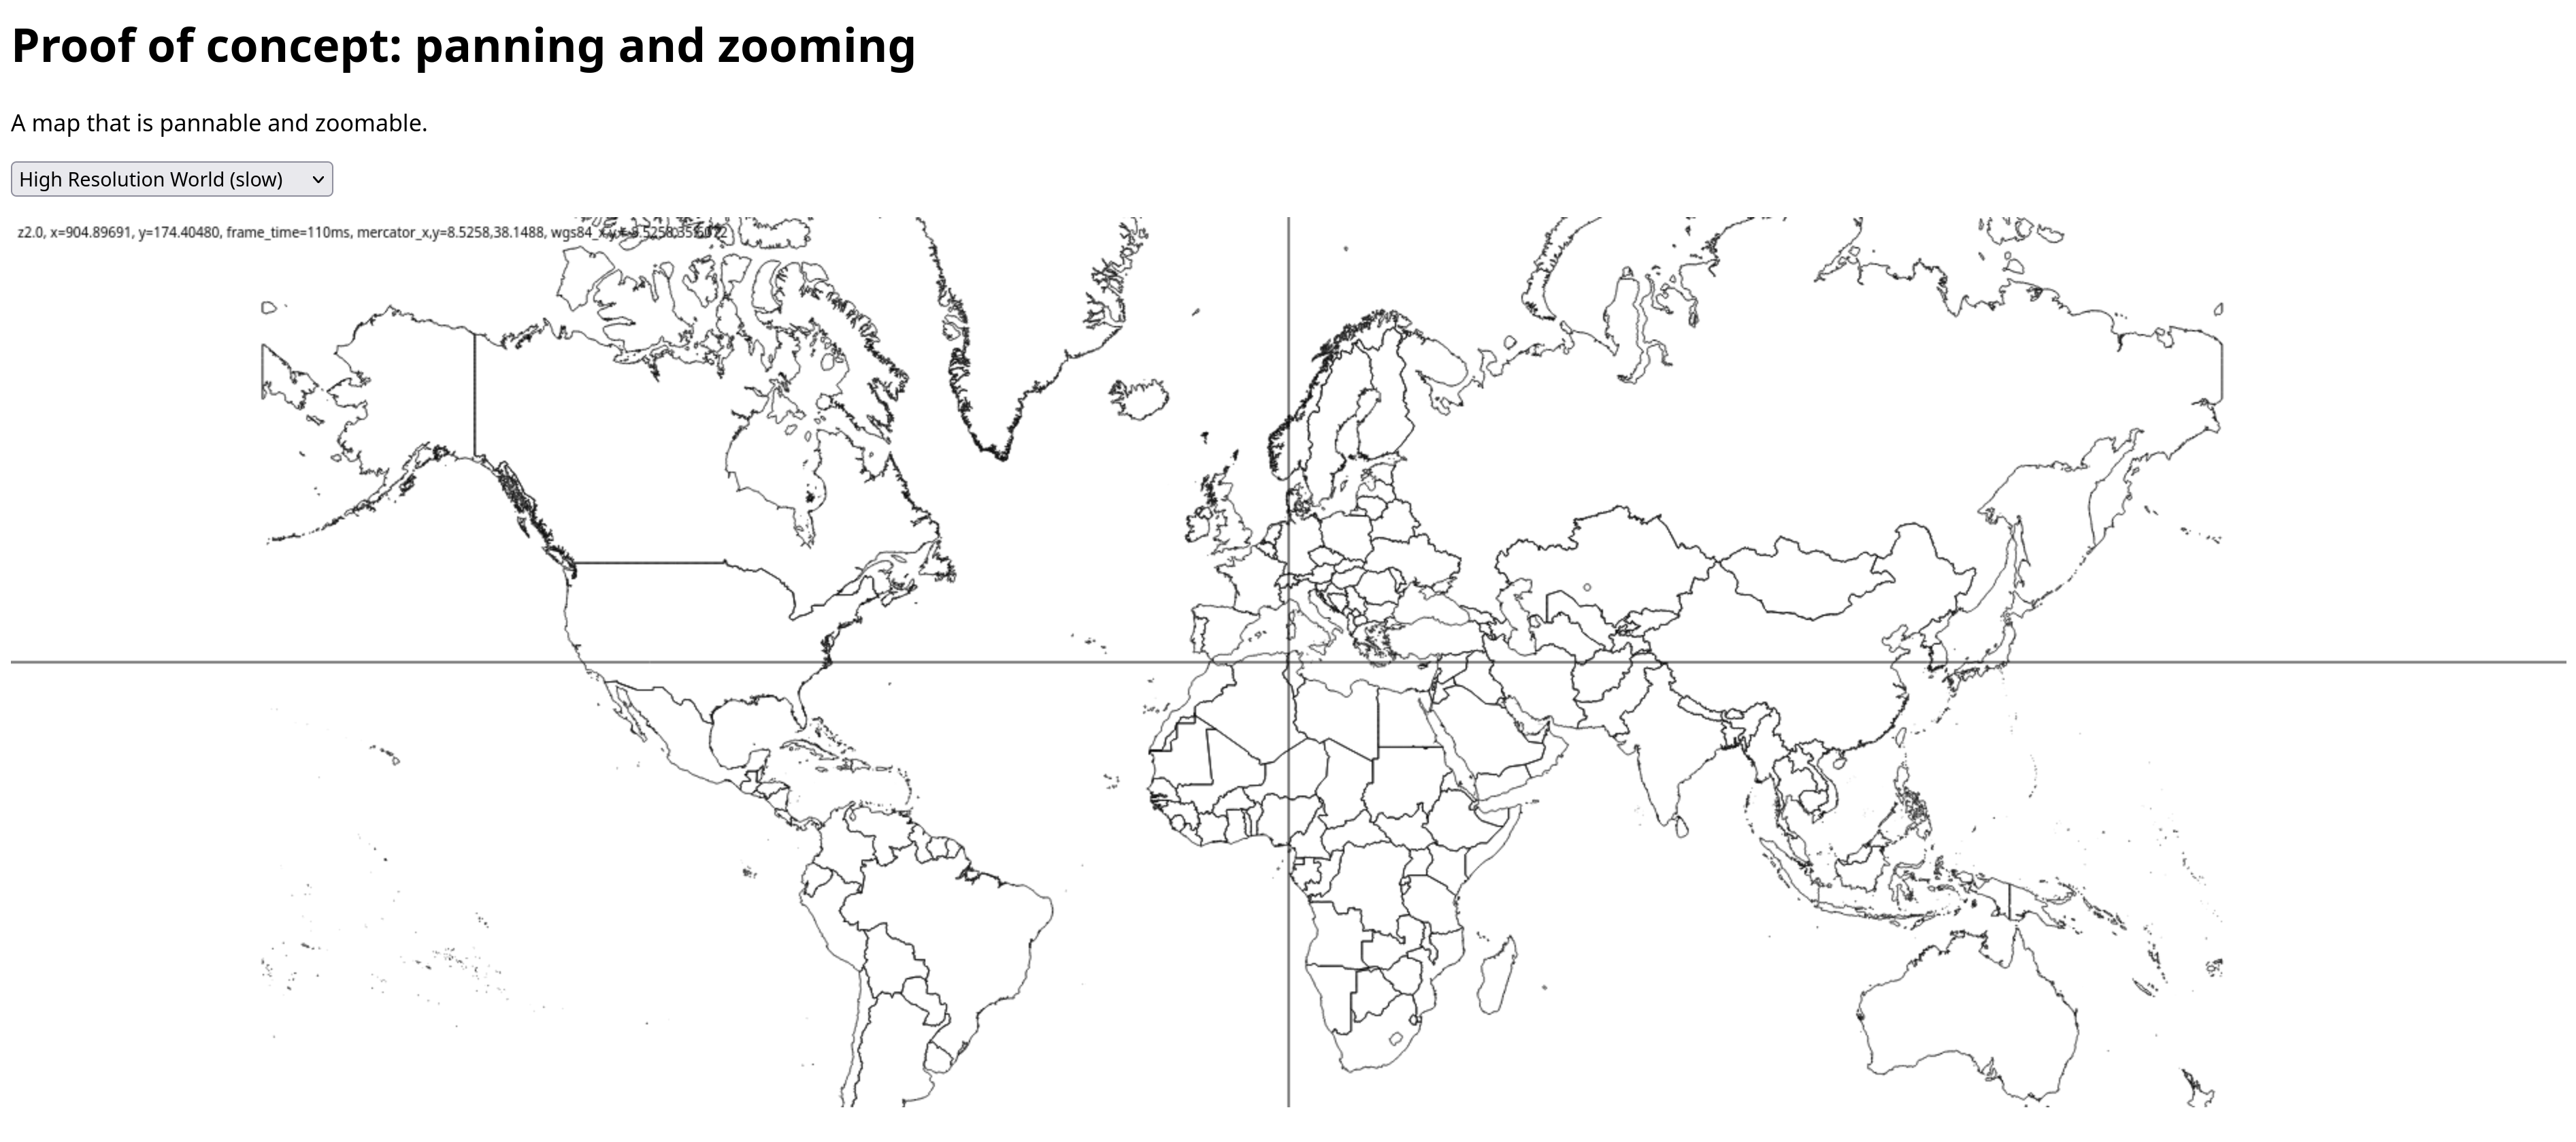
\includegraphics[width=\textwidth]{../proof-of-concepts/3-panning-and-zooming/screenshots/the-world.png}
    \caption{An interactive world map, using Natural Earth data~\cite{natural-earth}}
\end{figure}\label{fig:panning-and-zooming}

For testing the zooming between low and high zoom, I needed some ``large scale'' data to supplement the localized OSM data that I had downloaded for the previous proof of concept. Natural Earth Cultural Vector data seemed suitable, as it is readily available as GeoJSON, is released in the public domain, and is suitably low-detail for my purpose~\cite{natural-earth}. Once again I used \texttt{geojson.io}~\cite{geojson.io}, this time to merge these two sets of data.

To begin with, I was simply redrawing the map every time a \texttt{Touch} or \texttt{Mouse} event fired. This worked, but these events would often fire very rapidly (>60 times/second), resulting in a slow panning experience, where rendering was occurring unnecessarily. My solution for this was \texttt{requestAnimationFrame()}, which allows you to have some function executed at a regular interval by the browser~\cite{mdn-request-animation-frame}. Therefore, I could to modify the state of the map, then have it smoothly rendered at regular intervals to reflect any changes to zoom or offsets.

Unfortunately this change meant the canvas re-rendered 60 times a second at all times, even when no state change had occurred, which is a waste of processing power and energy, especially on mobile devices. To remedy this I introduced a \texttt{dirty} flag, which I set whenever a state change had occurred, checking it at the beginning of the \texttt{render()} function. The end result was a map that updated smoothly 60 times a second when state changes were occurring, and not at all when the map was static.

\begin{lstlisting}[caption=Only rendering when the map state is \texttt{dirty}]
public render() {
    // if nothing has changed, don't bother re-rendering
    if (!this.dirty) {
        requestAnimationFrame(() => this.render());
        return;
    }
    this.dirty = false;
    [...]
}
\end{lstlisting}

\section{Rendering tiled data from a Mapsforge file}

{ \footnotesize Source in \texttt{proof-of-concepts/4-rendering-osm-data}, or online demo at \href{https://files.george.honeywood.org.uk/4-rendering-osm-data/#15/50.7895/-1.8938}{\nolinkurl{files.george.honeywood.org.uk/4-rendering-osm-data/}}.}

My final proof of concept revolved around reading tiled vector OSM data. This allows for a map viewer that is performant at a wide range of zoom levels, as it can switch to more detailed data as you zoom in, and less detailed as you zoom out. It also solves the issue of which data to render --- my previous proof of concepts rendered all the data, all the time, even if it was off canvas. With tiled data, you only have to render the tiles that are currently within the viewport.

The bulk of the work for this proof of concept came in the form of writing a parser for the Mapsforge format~\cite{mapsforge-format}. I decided to use this format based on my report on OpenStreetMap data sources, in Section~\ref{sec:osm-data-sources}. This was because it seemed simpler to parse than the MBTiles, which is the other popular choice for tiled vector map files. It is a binary format, that is designed to space-efficiently encode geographical data, such that can be rendered on low-power mobile devices.

\subsection{The Mapsforge format}

Here I will explain the main concepts of the Mapsforge format, that I had to understand whilst writing the parser. This information is mostly as per the specification~\cite{mapsforge-format}, supplemented by what I learnt as I progressed.

\subsubsection{Points of Interest (PoIs)}

These represent tagged OpenStreetMap nodes, such as shops, bus stops, or any other objects that have been mapped as a node. They are also used for city/town/place labels at low zoom levels.

\subsubsection{Ways}

Ways are an abstraction over OpenStreetMap ways and relations, presenting both as a single type. OSM represents complex structures such as buildings with internal courtyards as multiple ways, for the outer and inner parts. These are then linked by a multipolygon relation that labels each part as inner or outer~\cite{osm-wiki-multipolygon}. These are non-trivial to efficiently interpret, especially with large amounts of data, so it makes sense to push this complexity to the map-writer software.

\subsubsection{Sub-files}

\begin{figure}[ht]
    \centering
    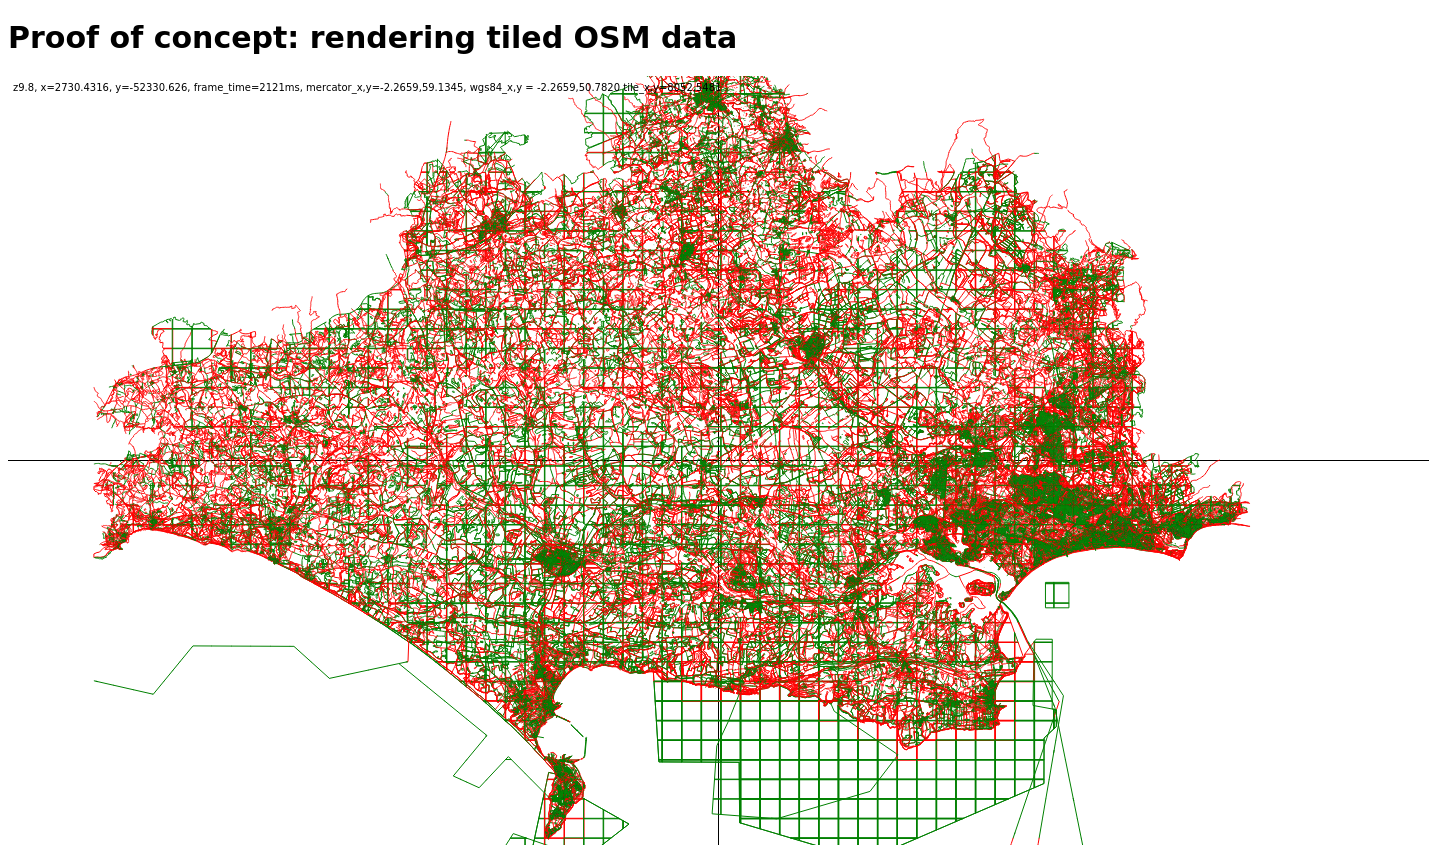
\includegraphics[width=0.8\textwidth]{../proof-of-concepts/4-rendering-osm-data/screenshots/high-detail-at-low-zoom.png}
    \caption{Raw tiled data from zoom 14 base tiles}
\end{figure}\label{fig:rendering-tiles}

%% \- to give latex line break hints

Sub-files store map data for a range of zoom levels. For example, the file \texttt{proof\--of\--concepts/4\--rendering\--osm\--data\-/data/ferndown.map} is compromised of three sub-files, one for z1-z7, based at z5, another for z8-z11, based at z10, and a final one for z12-z21, based at z14. This system provides a compromise between storage space and geographical correctness --- if say we want data for z18, we ``over-zoom'' the z14 sub-file, and vice versa for z1, we ``under-zoom'' the z5 sub-file. Therefore, we don't need to store much duplicated data, compared to storing each zoom level separately.

The over-zoom/under-zoom functionality is supported by each sub-file containing a ``zoom table'', which contains how many PoIs/Ways need to be read for the tile at the requested zoom level. For example, when under-zooming a z14 tile to z12, is very slow to render absolutely all the map features, as you will be showing around 112 z14 base tiles (on a 1080p screen). For the zoom-table to work, the Way and PoI data in each tile is sorted by ``feature importance'', meaning that data to be shown at low zoom levels, like place labels or important roads, comes first, and less important geometries like houses are placed last. Therefore, you can read that there should be \texttt{x} amount of PoIs/Ways for this tile, for the zoom level you are decoding, read the specified amount, then skip over the rest.

\subsubsection{Variable length integers}

To save file space, coordinates and other numbers are encoded in a custom format. This means that both large and small numbers can use the same representation, whilst requiring a minimal amount of bytes to store them. The format is based around the idea that the first bit of a byte is used as a continuation bit --- i.e., the \texttt{1000 0000} it is set in this byte. If the continuation bit is set, you continue to read the next byte as part of the same number.

The format is little-endian, meaning that the first byte of the number is the least significant\footnote{Note that the bytes themselves are still stored in big-endian format}. Hence, you can read whole number by shifting each of the subsequent numbers by \(7n\), then applying a bitwise \texttt{OR / |} against the current total.

\begin{lstlisting}[caption=Parsing variable length integers]
// decode a variable length unsigned integer as a number
getVUint() {
    // if the first bit is 1, need to read the next byte rest of the 7 bits
    // are the numeric value, starting with the least significant
    let value = 0;
    let shift = 0;

    // check if we need to continue
    while ((this.data.getUint8(this.offset) & 0b1000_0000) != 0) {
        // if this not the first byte we've read, each bit is worth more
        value |= (this.data.getUint8(this.offset) & 0b0111_1111) << shift
        this.offset++
        shift += 7
    }

    // read the seven bits from the last byte
    value |= (this.data.getUint8(this.offset) << shift)
    this.offset++
    return value
}
\end{lstlisting}

Signed integers follow a similar scheme with the continuation bit, but also sacrifice the second bit of the last byte to indicate the sign of the number, i.e., \texttt{0100 0000}. There is no concept of a floating point number in the format. Instead, you divide numbers when it is required, for example for coordinates, which are stored in the file in microdegree units.

\subsection{Writing a parser}

In my first iteration of this proof of concept, I was decoding the file inline, using a \texttt{DataView}, manually keeping track of offsets within the blob. This worked, but led to a lot of duplicate code that was just handling offsets, and a number of error caused by me making some trivial mistake when incrementing the offset by the wrong amount. To remedy this smell, I refactored the code to use the abstraction of a \texttt{Reader}. You construct the \texttt{Reader} with a blob, then call methods like \texttt{.getVUint()}, or \texttt{.getBigUint64()}. These methods increment an offset internal to the \texttt{Reader} class.

\subsection{Rendering the tiles}

\begin{figure}[ht]
    \centering
    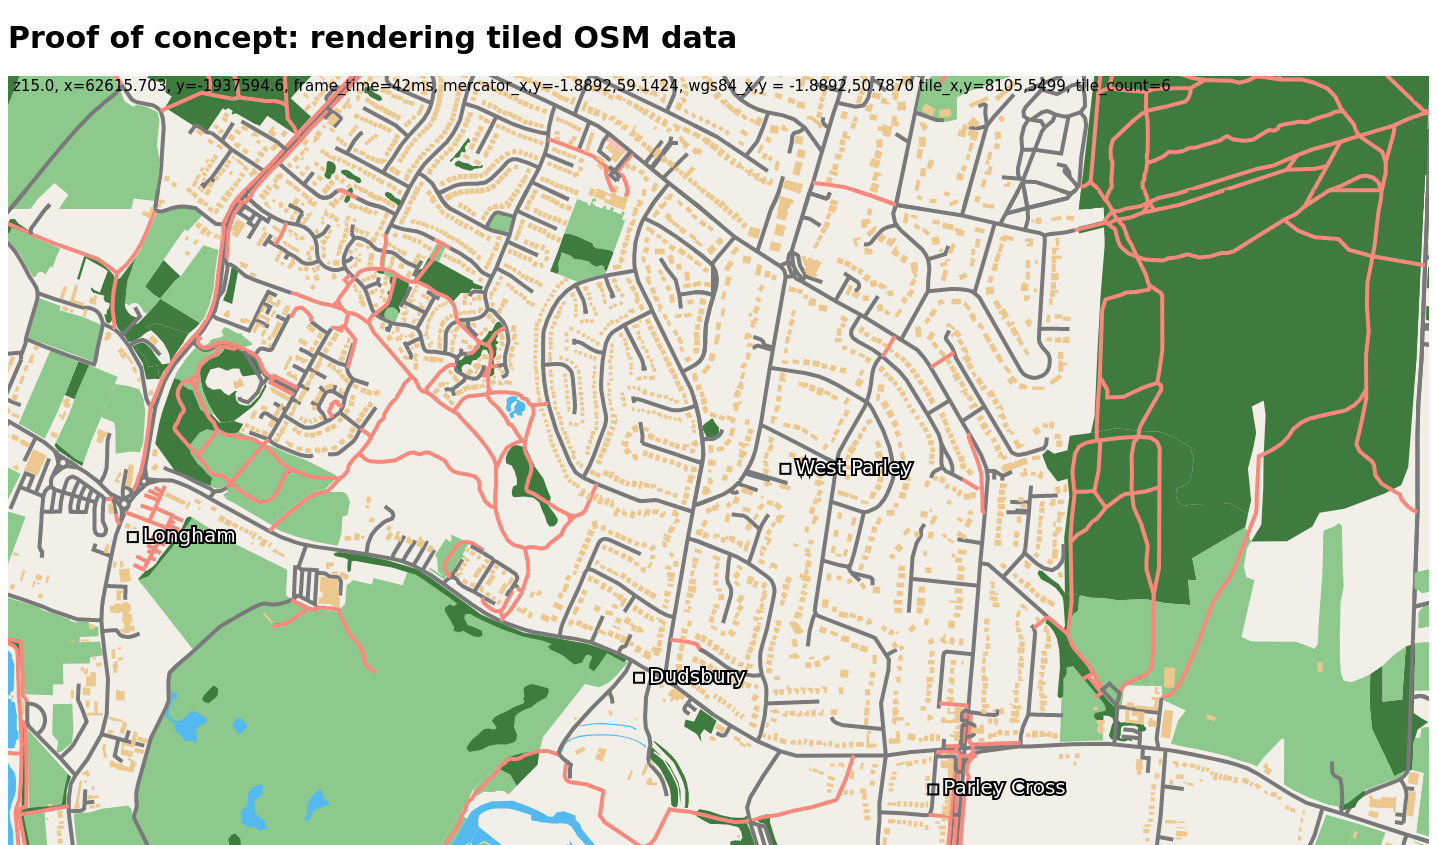
\includegraphics[width=\textwidth]{../proof-of-concepts/4-rendering-osm-data/screenshots/styled.png}
    \caption{Styling of data from Mapsforge file}
\end{figure}\label{fig:rendering-osm-data}

When rendering the map, I first convert the current zoom level to the corresponding base zoom level of one of the sub-files. Once I have this I then calculate the coordinates at the top-left and bottom right of the screen, then convert these into Z/X/Y tile numbers, which I can then fetch from the file. To improve rendering performance, only the PoIs and Ways specified in the zoom table for that zoom level are shown.

I handled styling fairly simplisticly, setting a number of booleans based on way tags as the tiles are loaded. This moves the more complicated (and slow) logic out of the rendering hot path. Inside the \texttt{render()} function I then check these booleans and choose whether a stroke or fill should be used for that way, and what colour it should be.

In order to make sure that labels are drawn on top, I make two passes through the data. First I render out all the areas and lines, then the way labels and PoIs. Before I implemented this, labels were being overlapped by areas from other tiles.

\chapter{Software engineering}

% convential commit messages
% talk about typescript

In order to successfully deliver a project, it is important to follow good software engineering practices. These should help you create something that has minimal technical debt, is correct, is maintainable, and can be easily understood by other members of a team.

I decided to write my project in TypeScript over plain JavaScript, as it provides an extremely helpful layer to help solve runtime type issues. It also allows my IDE, Visual Studio Code, to provide far more useful suggestions, compared to writing JS\@. This is because it is aware what types variables are at all times, instead of using a fallible heuristic approach.

Conveniently, the JavaScript bundler I chose, \texttt{esbuild}, has built in support for stripping TypeScript annotations, meaning I only have a single build step. It doesn't have the ability to check types itself, but this was not an issue for me, as VS Code performs this function natively in the editor. \texttt{esbuild} also has a convenient ``dev-server'' mode, where it bundles up the latest code as the requests come in, removing the need for a file-watcher.

\section{Testing}

Testing is critical to producing a piece of software that works as expected. It helps you to define what your function should return before you write it, and ensures that the function returns exactly what you expect.

In my project a significant amount of the work is rendering data to the HTML5 canvas. This portion of the project is very difficult to test --- at least while development is still occurring. Therefore, I directed my testing efforts towards the non-visual portions of the application, such as parsing the Mapsforge file, geometry operations, and projecting data.

I implemented testing using the Jest framework. Initially I had some issues setting it up to be able to understand tests and code written in TypeScript. Once it was set up, it was irritatingly slow, taking 5+ seconds to run with only a single test. The cause of this was two-fold; I was using the \texttt{ts-jest} package, which uses Babel to transpile TypeScript to JS (which is slow), and I had written my \texttt{jest.config.ts} in TypeScript. This meant that when I ran \texttt{jest test}, it had to spin up \texttt{ts-node} to interpret the file, which is also relatively slow. To fix this I rewrote the config file in plain JavaScript, and switched Jest to use \texttt{@swc-node/jest} instead of \texttt{ts-jest} to transpile the JavaScript, which reduced the time taken to under 2 seconds for the whole suite.

\begin{figure}[ht]
    \centering
    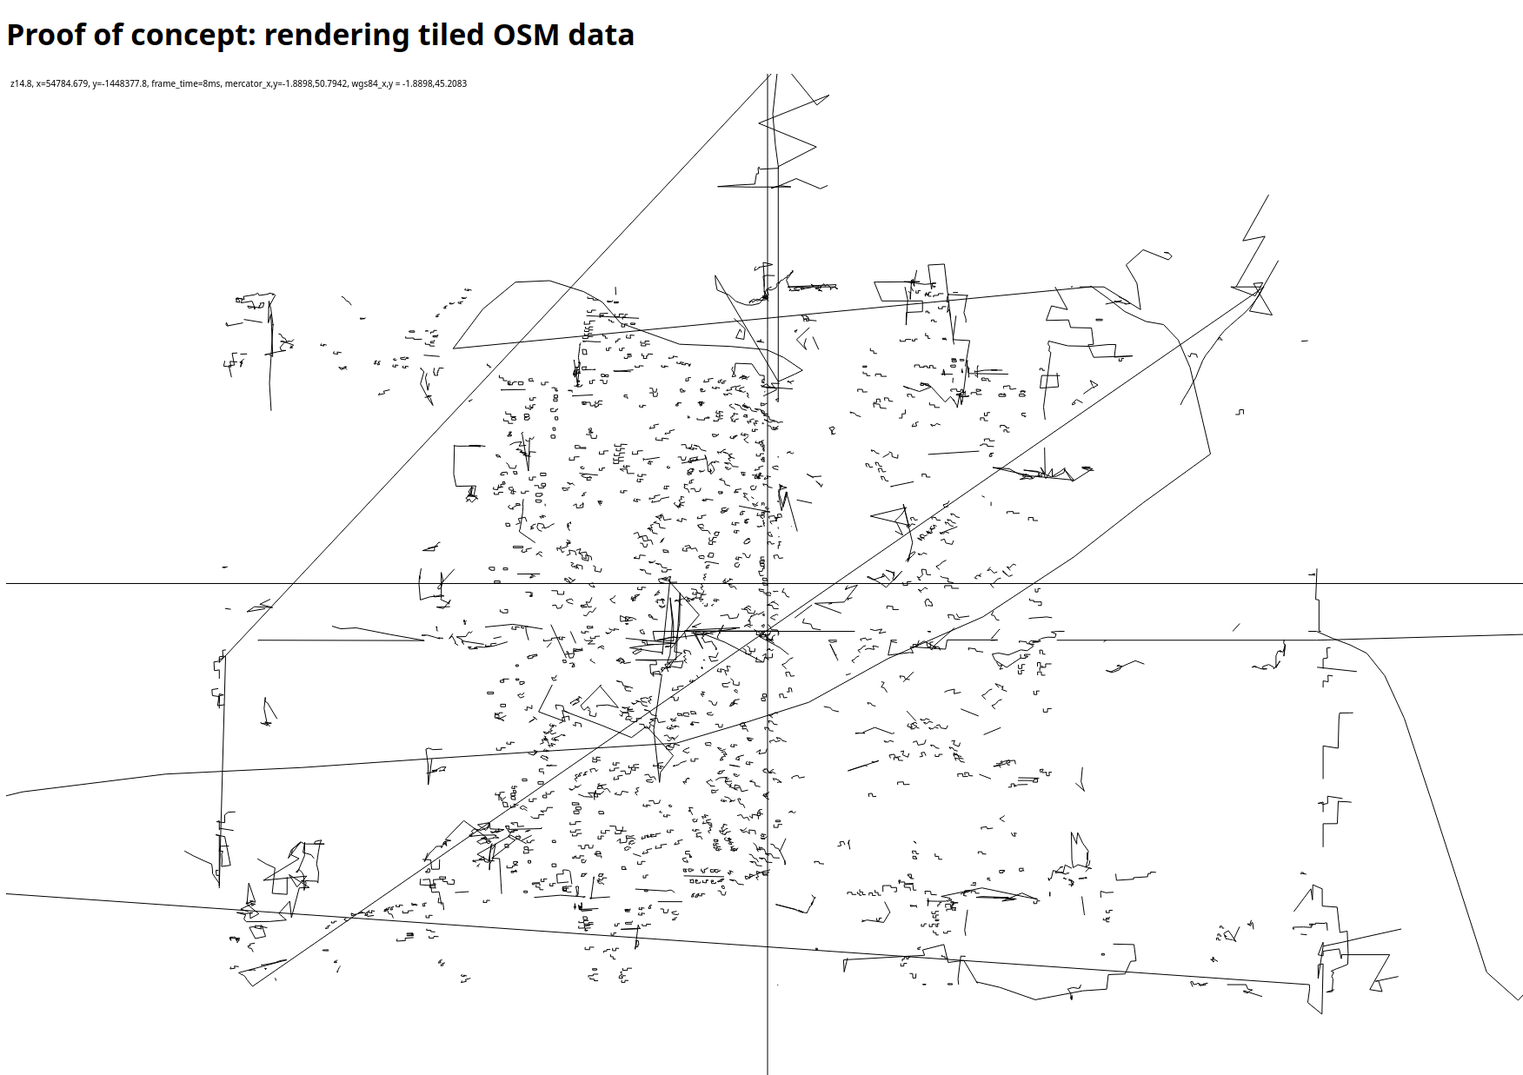
\includegraphics[width=0.8\textwidth]{../proof-of-concepts/4-rendering-osm-data/screenshots/artifacts.png}
    \caption{Rendering incorrectly parsed geometries}
\end{figure}\label{fig:artifacts}

In particular the tests for the \texttt{Reader} class proved very useful. At first, I didn't write any formal tests for the \texttt{.getVSint()} method --- instead running it and checking if the output seemed reasonable. This got me so far, with it returning some well-formed data, but when it came to rendering the geometries were all corrupted, as in~\ref{fig:artifacts}. During the debugging process, I wrote exhaustive table tests for this function, and I realized that I was incrementing my offset through the file on the wrong line.

\begin{lstlisting}[caption=Output from the \texttt{.getVSint()} test suite, numbers=none]
should be able to decode signed variable ints
    pass: 1 byte max negative: [01111111].getVSint() == -63
    pass: 1 byte max positve: [00111111].getVSint() == 63
    pass: 2 byte min: [10000000,00000001].getVSint() == 128 (1 ms)
    pass: 2 byte max: [11111111,01111111].getVSint() == -8191
    pass: 3 byte min: [10000000,10000000,01000001].getVSint() == -16384
    pass: 3 byte max: [11111111,11111111,01111111].getVSint() == -1048575
    pass: 4 byte min: [10000000,10000000,10000000,00000001].getVSint() == 2097152
\end{lstlisting}

\section{Version control}

Another important software engineering practice is making good use of version control.

\section{Documentation}

\section{Profiling}

%% for final report:
%\chapter{Final application development process}

\chapter{Conclusion}

%% for final report:
% \section{Professional issues}
% look on the BCS website for ideas

\section{Evaluation}

\chapter{Annexe}

%% include the full diary.md here.
%% could convert to .tex with pandoc

\addcontentsline{toc}{chapter}{Bibliography}

% smaller bibliography text
\renewcommand*{\bibfont}{\normalfont\small}
\printbibliography{}

\end{document}
